\item I\textsubscript{CM} is the moment of inertia of a circular disc about an axis (CM) passing through its centre and perpendicular to the plane of disc. I\textsubscript{AB} is it's moment of inertia about an axis AB perpendicular to plane and parallel to axis CM at a distance $\frac{2}{3}R$ from centre.

Where \( R \) is the radius of the disc. The ratio of \( I\textsubscript{AB} \) and \( I\textsubscript{CM} \) is \( x : 9 \). The value of \( x \) is \underline{\hspace{2.5cm}}.
    \begin{center}
        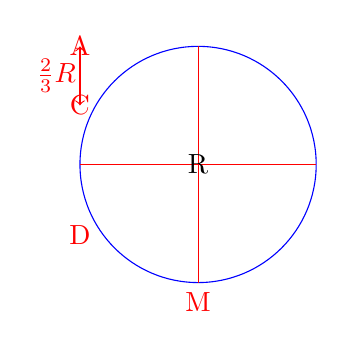
\begin{tikzpicture}
            \draw[blue] (0, 0) circle[radius=1.5];
            \draw[red] (-1.5, 0) -- (1.5, 0);
            \draw[red] (0, 1.5) -- (0, -1.5);
            \draw[red] (0, -1.5) node[anchor=north] {M};
            \draw[red, <->] (-1.5, 0.75) -- (-1.5, 1.5);
            \node[red] at (-1.8, 1.125) {\(\frac{2}{3}R\)};
            \node[red] at (-1.5, 1.5) {A};
            \node[red] at (-1.5, 0.75) {C};
            \node[red] at (-1.5, -0.9) {D};
            \node at (0,0) {R};
        \end{tikzpicture}
    \end{center}